\chapter{Testing and Evaluation}
\lhead{\emph{Testing and Evaluation}}
\label{chapter:eval}

For the purposes of fairly evaluating this system, three different aspects of it were tested: the quality of its 3D representation as an abstraction of the rover's space, its real-time performance, and its bandwidth compared to a non-abstraction based system. It should be noted that none of these are a direct evaluation of the presence the system provides, as the presence of a system is a fairly subjective assessment that would require studies of large user groups to evaluate with any accuracy. While this prevents direct evaluation, the potential for presence can be indirectly evaluated through the aspects that were tested.

\section{3D Model Quality}

The system's ability to produce recognisable representations of the rover's environment was tested in a lab environment, with encouraging results. Most objects were recognisable from their abstracted representations and placed at the correct depth in the scene (Figure \ref{fig:UDemos}). 

\begin{figure}[H]
    \begin{center}
    \begin{tabular}{ c c }
        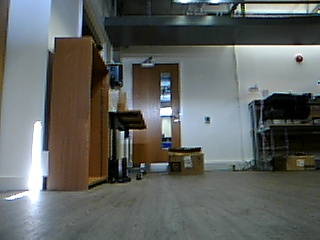
\includegraphics[width=0.43\textwidth,trim={0.5cm 0 1cm 0},clip]{Figures/TestScene1.jpg} &
        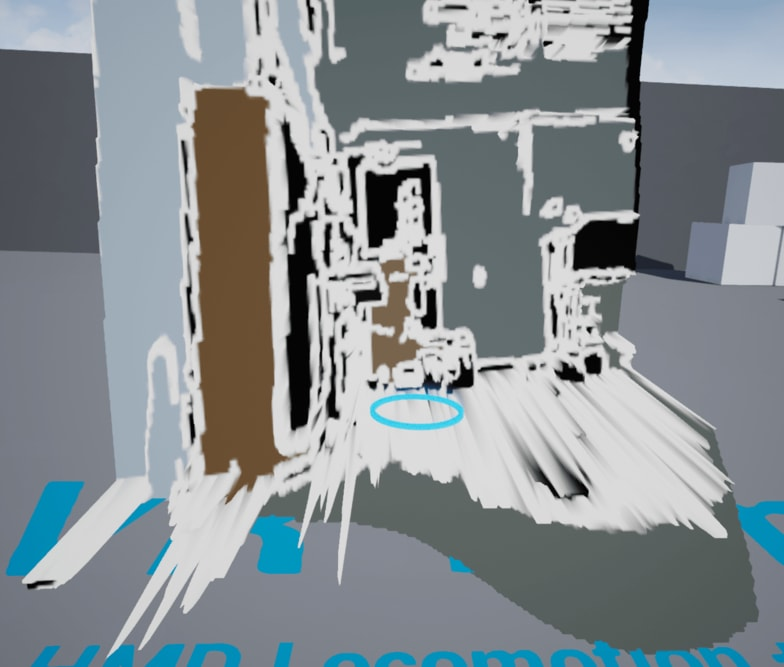
\includegraphics[width=0.43\textwidth]{Figures/TestUnreal1.jpg} \\
        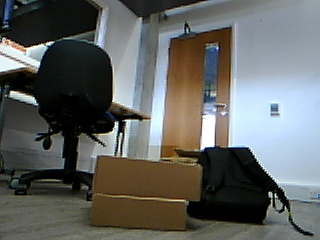
\includegraphics[width=0.43\textwidth,trim={0.5cm 0 1.5cm 0},clip]{Figures/TestScene2.jpg} &
        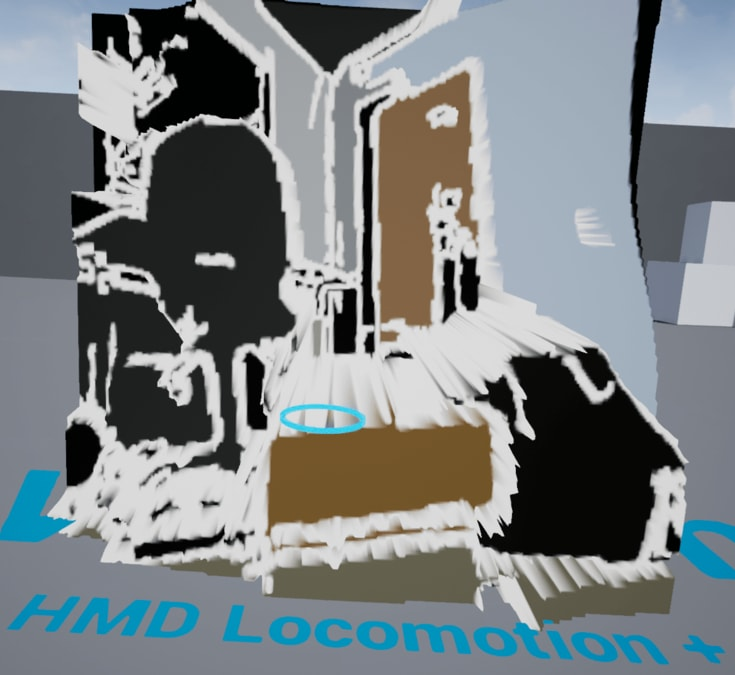
\includegraphics[width=0.43\textwidth]{Figures/TestUnreal2.jpg}
    \end{tabular}
    \caption[Full System Demonstrations]{Full System Demonstrations. The left images are of test scenes, the images taken at the resolution of the rover's cameras, and the right images are of the 3D representations of the test scenes. The scenes are clearly recognisable, with most objects at their correct depths such as the boxes and bag being at the front in the bottom right image. The issues with the system can also be seen, with the errors and odd floor position in the top right image.}
    \label{fig:UDemos}
    \end{center}
\end{figure}

It was found that objects with simple shapes, such as boxes, were represented with high accuracy, however the more complex the shape the less accurate the representation became. This is because the system does not detect changes in depth across the face of an object very well---depth is only calculated from the edges. This results in every object being represented as mostly flat, however, as predicted in Chapter \ref{chapter:abstract}, the user only needs the outline and average colour of an object to be able to recognise it, so object recognition is not significantly affected.

The issue of the floor being represented incorrectly in the depth map (discussed in Section \ref{section:depth}) remains an issue in the 3D model. For example, the dark grey section of the floor in the top right image of Figure \ref{fig:UDemos} should extend all the way to the back of the scene, instead it has been pushed forward as a large block at around ankle height. While it is most noticeable in the floor, the problem is actually a general inability to correctly produce depth maps of slanted surfaces from edge detected images---every surface in the scene will be represented as perpendicular to the camera. Due to this issue being based in the complexities of edge detection based depth mapping, solving it would require significant reworking of the mapping algorithm and filtering technique. However, it is also an issue that does not significantly impact the user under normal usage unless they explicitly attempt to look down at the floor.

The other issue noted at the depth mapping stage, the mistakes the algorithm makes with certain objects, also remains an issue in the 3D model. If an object is very thin, or contains parallel edges in close proximity to each other, it may be incorrectly placed significantly closer to the camera (Figure \ref{fig:UErrors}).

\begin{figure}[H]
    \begin{center}
    \begin{tabular}{ c c }
        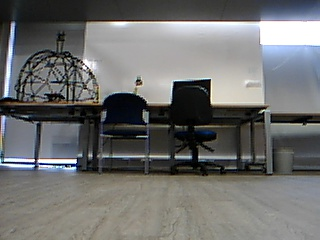
\includegraphics[width=0.43\textwidth,trim={0cm 0 1cm 0},clip]{Figures/TestScene3.jpg} &
        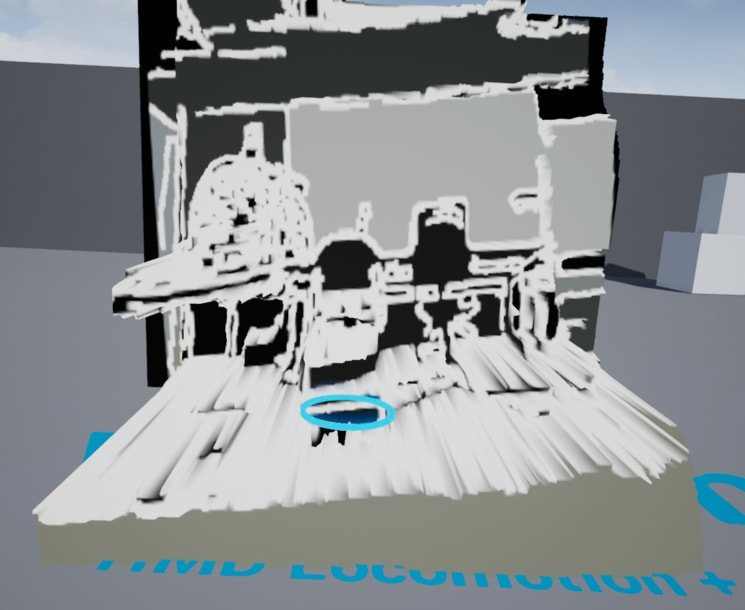
\includegraphics[width=0.43\textwidth]{Figures/TestUnreal3.jpg} \\
        \multicolumn{2}{c}{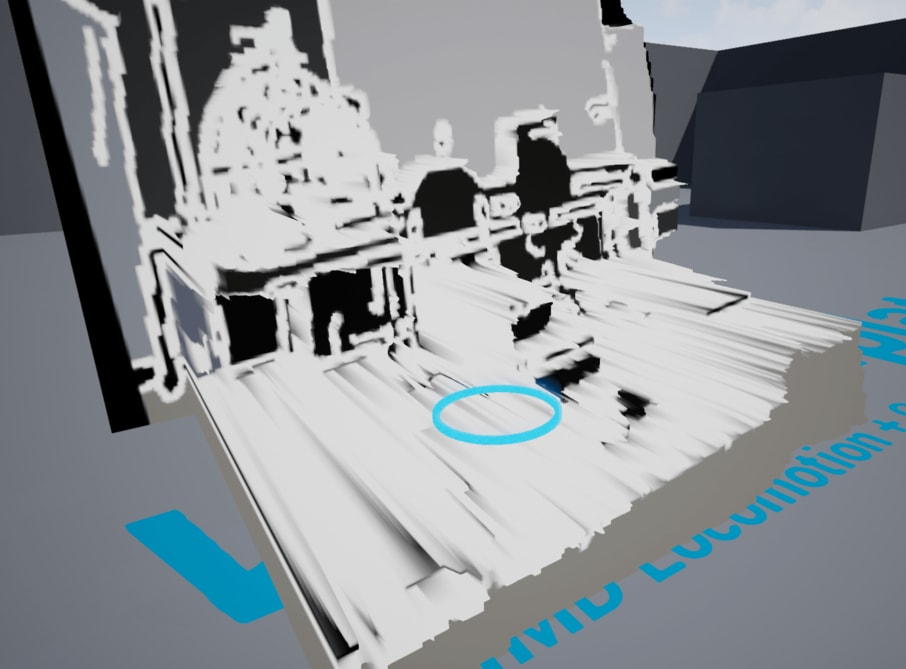
\includegraphics[width=0.5\textwidth]{Figures/TestUnreal3S.jpg}}
    \end{tabular}
    \caption[Demonstration of System Errors]{Demonstration of System Errors. The scene (top left) is very difficult for the system to reproduce, as it consists of thin, poorly lit objects. While the reproduction is recognisable, there are clear errors such as under the left chair and the left side of the table. The blue ellipses are once again UI elements that have no relevance to the 3D model, so should be ignored.}
    \label{fig:UErrors}
    \end{center}
\end{figure}

The errors are a by-product of using small images, as this results in thin objects often only being 5 or less pixels thick. With so few pixels representing them, its unsurprising these objects are not accurately placed in the depth map. The solution to this would be to use higher resolution images. This is not possible within the performance constraints of the R-Pi 3, though in a future iteration of the system where the R-Pi could be replaced with a higher performance option, it becomes entirely achievable.

\section{Run-Time Performance}

As intended, the VR headset maintains 90 fps and low latency regardless of how the rest of the system is performing. It is therefore unlikely that the user would feel motion sickness while using the system (no-one that tried it did), meaning the issue that prevents high levels of presence in most VR teleoperations systems has been successfully tackled. The rate the 3D model updates at is fairly consistently between 20 and 25 fps, and the latency of the system is generally between 0.25 and 0.5 seconds. The frame rate and latency are entirely dictated by the processing power of the rover, as this is the bottleneck of the system, therefore replacing the R-Pi 3 with a more powerful device would significantly improve these results.

At the present level of performance, controlling the rover through the 3D model is intuitive and comfortable. The latency does affect the user's ability to move the rover with precision, though not to a significant degree. The 3D model remains accurate regardless of the speed the rover moves forward or backwards at, however turning does have an impact on depth map accuracy. This is not a serious issue though, as the coloured abstraction texture remains accurate, even if the depth map does not, resulting in the user's awareness of the environment being largely unaffected.

\section{Comparison to a Non-Abstraction System}

The final aspect that required testing is whether the system has lower bandwidth requirements than similar systems that do not use data abstraction. A test non-abstraction system was built that sends 2 normal images over UDP, then attempts to generate a depth map from them. The lowest packet size that this system could produce while still generating depth maps comparable to the abstracted system was discerned by varying the level of JPEG compression applied to the images (Figure \ref{fig:packetc}).

\begin{figure}[H]
    \begin{center}
      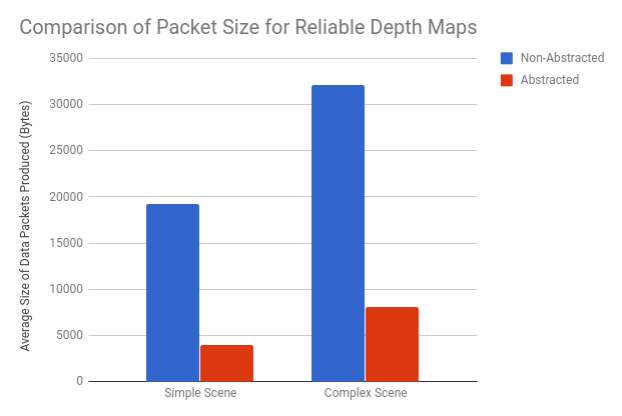
\includegraphics[width=0.7\textwidth]{Figures/packetcomp.png}
      \caption[Comparison of Packet Size for Reliable Depth Maps]{Comparison of Packet Size for Reliable Depth Maps. JPEG Compression was decreased until the non-abstraction system produced depth maps of comparable accuracy to the abstraction system.}
      \label{fig:packetc}
    \end{center}
\end{figure}

Attempting to reduce the packet size of the non-abstraction system to the maximum packet size observed from the main system results in depth maps that do not contain any useful information (Figure \ref{fig:absjpg}), leading to the conclusion that the system presented by this report does provide a significant reduction in the bandwidth requirements for VR teleoperations.

\begin{figure}[H]
    \begin{center}
      \begin{tabular}{ c c }
        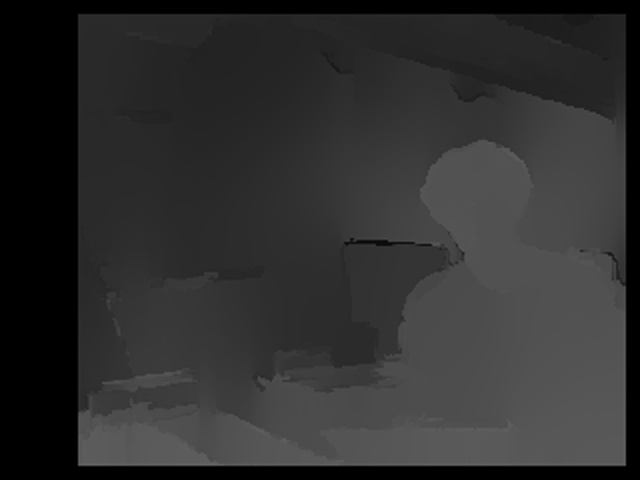
\includegraphics[width=0.47\textwidth]{Figures/abstest.jpg} &
        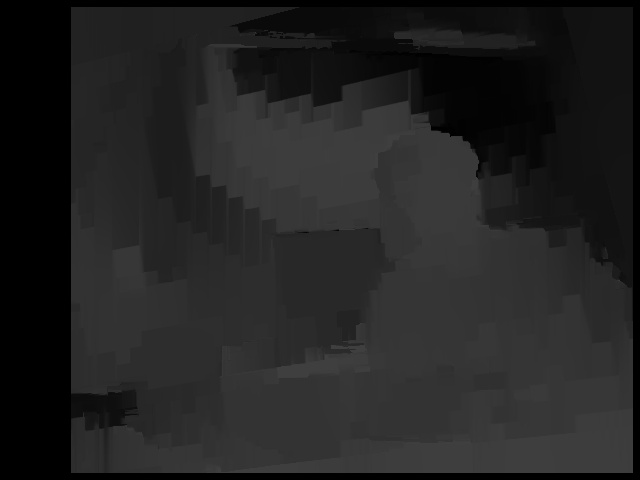
\includegraphics[width=0.47\textwidth]{Figures/jpgtest.jpg}
      \end{tabular}
      \caption[Non-Abstraction Depth Map Comparison at Equal Packet Size]{Non-Abstraction Depth Map Comparison at Equal Packet Size. At a packet size of roughly 5800 bytes, the abstraction system (left) produces clearly defined and accurate shapes with mostly correct depths, whereas the non-abstraction system (right) produces mostly noise, with little relation to the original scene.}
      \label{fig:absjpg}
    \end{center}
\end{figure}